\section{特殊的图}
\label{sec:graph-special-graphs}

一般图的连接结构千差万别，很多在一般图上难以判别或代价高昂的问题，一旦限制在满足特定全局约束的图族上，就会呈现出简洁的定量规律与高效的算法。本节聚焦三类最核心的特殊图：第~\ref{sec:graph-trees-forests}小节的树与森林禁止出现任何环，用最少的边维持连通；第~\ref{sec:graph-bipartite-graphs}小节的二部图要求顶点可划分为内部无边的两部分，等价于禁止出现奇环；第~\ref{sec:graph-planar-graphs}小节的平面图要求能在平面上不交叉地画出全部边，顶点数、边数与面数之间满足欧拉公式。

\subsection{树与森林}
\label{sec:graph-trees-forests}

第~\ref{sec:graph-conn-cut-bridge}小节看到，边位于环上时删掉它不会断开连接，环提供的是冗余的替代路径。若要用尽量少的道路把一组城市连起来，就不应保留任何环。本小节研究这种连通而无环的结构。树的两个条件分别对应路径的存在与唯一，由此能数出树的边数，边数又反过来给出判断树的简便方法。

此后两目讨论树的两种用法：在树上选根可以组织上下层次，在一般连通图中则可以抽出一棵覆盖全部顶点的树。这些结论是第~\ref{chap:graph-traversal}章遍历结果、第~\ref{sec:graph-minimum-spanning-tree}章最小生成树和第~\ref{sec:graph-tree-dp}节树上动态规划的共同基础。

\subsubsection{树与森林的定义}
\label{sec:graph-conn-tree-definition}

不修多余道路的道路网应当连通，以保证任意两点之间都有路线；还应当无环，因为由定理~\ref{thm:graph-conn-bridge-cycle}，环上的边删去后图仍然连通，可以省掉。同时要求这两点就得到树，只要求无环得到的是若干互不相连的树。

\begin{definition}[树与森林]
\label{def:graph-conn-tree}
非空、连通且不含环的无向图称为\term{树}（tree）。不含环的无向图称为\term{森林}（forest）。
\end{definition}

森林的每个连通分量都连通且无环，是一棵树；只有恰好一个分量的森林才是树。

图~\ref{fig:graph-conn-tree-forest}中，(a)的链和(b)的星形都是树，树可以有分支；(c)的三角形连通但有环，不是树；(d)有三个分量，每个都是树，整体是森林。

两个边界情形需要注意。只有一个顶点、没有边的图是单点树，所以树中的顶点不必都有邻边。空图不含环，是有$0$个分量的空森林，但树要求非空，所以空图不是树。

\begin{figure*}[!htb]
  \centering
  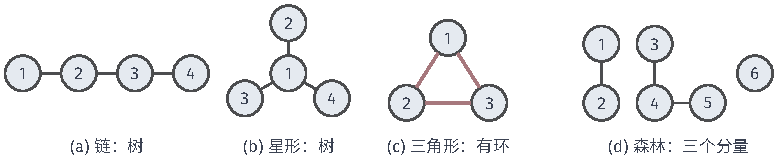
\includegraphics[scale=1]{figures/01-basic-mathematics/04-graphs/tikz/c1-tree-forest/figure.pdf}
  \caption{树、森林与非树的对照。(a)链与(b)星形都是树，后者有分支；(c)三角形连通但含有红色标出的环，不是树；(d)由三个互不相连的树组成的森林，其中孤立顶点$6$是一棵单点树。}
  \label{fig:graph-conn-tree-forest}
\end{figure*}

\subsubsection{树的基本性质}
\label{sec:graph-conn-tree-properties}

\paragraph{路径唯一性}
树的连通保证任意两点之间有路径，无环则保证这样的路径只有一条。直观上，若两点之间有两条不同的路径，它们分开以后终究要会合，分开与会合之间的两段就围成一个环；反过来，环上相邻的两点既有一条边直接相连，又可以沿环的另一侧到达。

\begin{theorem}[树中路径唯一]
\label{thm:graph-conn-tree-unique-path}
设$\mathcal G$是非空无向图。$\mathcal G$是树，当且仅当任意两个顶点之间恰有一条路径。
\end{theorem}

\begin{proof}
先设$\mathcal G$是树。连通性保证任意两点$u,v$之间至少有一条路径。假设有两条不同的路径$P=(p_0,\ldots,p_a)$与$Q=(q_0,\ldots,q_b)$，$p_0=q_0=u$，$p_a=q_b=v$。一条不能是另一条的真前段，否则较长的那条会两次经过$v$；所以存在最小的$s$使$p_{s+1}\neq q_{s+1}$，记$x=p_s=q_s$。由于$v$同时在两条路径上，可以取$P$在$x$之后第一个也出现在$Q$中$x$之后的顶点$y$。

$P$从$x$到$y$的一段与$Q$从$x$到$y$的一段除端点外没有公共顶点：$P$这一段的中间顶点按$y$的取法不在$Q$中$x$之后的部分，又因为$P$是路径，也不在两者共有的$x$之前的部分。沿$P$从$x$走到$y$，再沿$Q$倒着走回$x$，得到一个除首尾外不重复顶点的闭行走。两段不能都只有一条边，否则$p_{s+1}=y=q_{s+1}$；所以它的长度至少为$3$，是一个环，矛盾。图~\ref{fig:graph-conn-tree-properties}画出了这个构造。

反过来，设任意两点之间恰有一条路径，则$\mathcal G$连通。若$\mathcal G$含环$(c_0,c_1,\ldots,c_{k-1},c_0)$，$k\geq3$，则$(c_0,c_1)$与$(c_0,c_{k-1},\ldots,c_1)$是从$c_0$到$c_1$的两条不同路径，矛盾。
\end{proof}
\begin{BookInlineFigure}
  \centering
  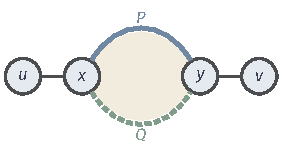
\includegraphics[scale=1]{figures/01-basic-mathematics/04-graphs/tikz/c1-tree-properties/figure.pdf}
  \caption{两条不同路径会围出环。路径$P$（蓝色实线）与$Q$（绿色虚线）在$x$分开、在$y$第一次会合；它们之间的两段构成黄色区域的边界，因此树中不可能同时存在这两条路径。}
  \label{fig:graph-conn-tree-properties}
\end{BookInlineFigure}

由这个定理，删除树的任意一条边$e=\{u,v\}$后$u,v$之间不再有路径，由定理~\ref{thm:graph-conn-bridge-cycle}，树恰好分成两棵较小的树。树的每条边都是桥。

\paragraph{边数}
数树的边数要用到度为$1$的顶点，称为\term{叶}（leaf）。叶只与一个顶点相连，删掉它不会断开其余部分，这使我们能对顶点数归纳。先说明叶总是存在。

\begin{lemma}[树有叶]
\label{lem:graph-conn-tree-leaves}
至少有两个顶点的树至少有两个叶。
\end{lemma}

\begin{proof}
取一条最长的路径$P=(v_0,\ldots,v_k)$，由于树连通且至少有两个顶点，$k\geq1$。若$v_0$另有邻居$z\neq v_1$：$z$不在$P$上时，$(z,v_0,\ldots,v_k)$是更长的路径；$z=v_t$在$P$上时$t\geq2$，$(v_0,v_1,\ldots,v_t,v_0)$是环。两种情形都不可能（图~\ref{fig:graph-conn-tree-properties-leaf}），所以$d_{v_0}=1$。同理$d_{v_k}=1$。
\end{proof}
\begin{BookInlineFigure}
  \centering
  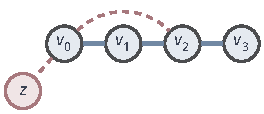
\includegraphics[scale=1]{figures/03-graphs/01-structure-and-computation/tikz/tree-longest-path-leaf/figure.pdf}
  \caption{最长路径的端点必须是叶。若端点$v_0$另有邻居，邻居在路径外（如$z$）会使路径延长，在路径上（如$v_2$）则会形成环；红色虚线表示这两种不可能的连接。}
  \label{fig:graph-conn-tree-properties-leaf}
\end{BookInlineFigure}

\begin{theorem}[树的边数]
\label{thm:graph-conn-tree-edges}
有$n$个顶点的树恰有$n-1$条边。
\end{theorem}

\begin{proof}
对$n$归纳，$n=1$时单点树没有边。设$n\geq2$，由引理~\ref{lem:graph-conn-tree-leaves}，树$\mathcal T$有一个叶$v$。$\mathcal T-\{v\}$无环；它也连通，因为路径的中间顶点要有两条路径上的邻边，度为$1$的$v$不会出现在连接其他两点的路径中间。所以$\mathcal T-\{v\}$是$n-1$个顶点的树，有$n-2$条边，加上$v$的那条边得$n-1$条。
\end{proof}

\subsubsection{树的判定}
\label{sec:graph-conn-tree-test}

按定义判断一张图是不是树，要确认它没有环，而这是关于全部顶点序列的断言。边数定理提示了另一条途径：数一下边，再查一次连通。为此先说明任何连通图都能用$n-1$条边连成一棵树。

构造从一个顶点出发，每次向外多接一个顶点。任取顶点$r$，令$S=\{r\}$、$F=\varnothing$。只要$S\neq V$，就取$S$外的顶点$t$和一条从$r$到$t$的路径，路径上必有一步从$S$内走到$S$外，把这一步的边加入$F$、它的$S$外端点加入$S$。每一步增加一个顶点和一条边，$n-1$步后$S=V$，$|F|=n-1$。

这样选出的$(V,F)$是树。它连通，因为每个新顶点都连到先前的顶点。它也无环：若$F$中有环，取环上最后加入$S$的顶点$t$，它在环上的两个邻居都更早加入；而$F$中$t$与更早顶点之间的边只有$t$加入时选出的那一条，矛盾。

\begin{theorem}[连通且$n-1$条边的图是树]
\label{thm:graph-conn-connected-tree-test}
设$\mathcal G$是有$n\geq1$个顶点的连通无向图。若$\mathcal G$恰有$n-1$条边，则$\mathcal G$是树。
\end{theorem}

\begin{proof}
按上面的构造选出树$(V,F)$。$F\subseteq E$且$|F|=n-1=|E|$，所以$F=E$。
\end{proof}

\paragraph{森林的边数}
设森林有$n$个顶点、$c$个分量，第$k$个分量有$n_k$个顶点。每个分量是树，有$n_k-1$条边，所以森林的边数是
\begin{equation}
\sum_{k=1}^{c}(n_k-1)=n-c.
\label{eq:graph-conn-spanning-forest-edges}
\end{equation}
于是无环且有$n-1$条边的图只有一个分量，也是树。

\paragraph{三个条件的关系}
对$n\geq1$个顶点的无向图，连通、无环、恰有$n-1$条边三个条件中，前两个由定理~\ref{thm:graph-conn-tree-edges}推出第三个，连通与$n-1$条边由定理~\ref{thm:graph-conn-connected-tree-test}推出无环，无环与$n-1$条边由式\eqref{eq:graph-conn-spanning-forest-edges}推出连通。

只有一个条件不够：三角形加一个孤立顶点（图~\ref{fig:graph-conn-components}(a)）有$4$个顶点、$3$条边，却既不连通又有环。

所以判断树只需两步：若$m\neq n-1$，立即否定；否则查连通。

例如边集为$\{1,2\},\{1,3\},\{1,4\},\{2,5\},\{3,6\}$的六点图有$5=n-1$条边，从$1$出发能到达全部顶点，所以是树；贯穿图有$5\neq3$条边，第一步就被排除。在大图上，第二步由第~\ref{sec:graph-connectivity-computation}节的连通分量计算完成。

\subsubsection{有根树}
\label{sec:graph-conn-rooted-trees}

家谱、文件目录或分治计算中，每个顶点有一个上级、可能有若干下级，无向树的边却读不出谁是上级。路径唯一性使我们可以从任意一个顶点出发组织这样的层次。

在树$\mathcal T$中选定一个顶点$r$作为根，得到\term{有根树}（rooted tree）。对每个$v\neq r$，从$r$到$v$的唯一路径上紧挨在$v$之前的顶点称为$v$的\term{父节点}（parent），$v$称为它的\term{子节点}（child）。从$r$到$u$的路径经过$v$的那些顶点$u$（包括$v$本身）组成以$v$为根的\term{子树}（subtree）。在有根树中，没有子节点的顶点称为叶。

\paragraph{父子关系的确定}
不必逐个找路径，可以一层层确定：根的邻居都以根为父节点；此后每确定一个顶点$u$的父节点，就把$u$除父节点以外的邻居都定为$u$的子节点。依据是：这样的邻居$w$不在从$r$到$u$的路径上，否则会与边$\{u,w\}$构成环，所以那条路径接上$w$就是从$r$到$w$的唯一路径。

图~\ref{fig:graph-conn-tree-properties-roots}的树有边$\{1,2\},\{1,3\},\{3,4\},\{3,5\}$。以$1$为根时，$2,3$的父节点是$1$，$4,5$的父节点是$3$，叶是$2,4,5$；以$4$为根时，$3$的父节点是$4$，$1,5$的父节点是$3$，$2$的父节点是$1$，叶是$2,5$。根$4$在无向树中是叶，在以它为根的有根树中却不是。第~\ref{chap:graph-traversal}章的遍历在树上给出的就是这样的父子关系。

\begin{BookInlineFigure}
  \centering
  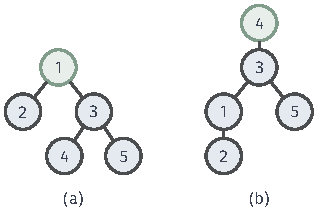
\includegraphics[scale=1]{figures/03-graphs/01-structure-and-computation/tikz/tree-root-choice/figure.pdf}
  \caption{同一棵树的两种选根。(a)以$1$为根，叶是$2,4,5$；(b)以$4$为根，叶是$2,5$。绿色顶点是根，边集不变，父子关系和有根树的叶集合随根改变。}
  \label{fig:graph-conn-tree-properties-roots}
\end{BookInlineFigure}

选根没有增删任何边，只规定每条边上哪一端是父节点；记录$n-1$个非根顶点的父节点就能还原边集，换一个根则全部重新确定。把每条边定向为从父节点指向子节点，得到一张有向图，但这一方向来自选根，而一般有向图的弧方向是原始数据，两者不应混同。第~\ref{sec:graph-tree-dp}节在有根树上自下而上计算时，利用的正是“每个子树只通过它的根与外界相连”。

\subsubsection{生成树与生成森林}
\label{sec:graph-conn-spanning-trees}

道路网中常要选出一部分道路，使所有城市仍然连通且没有多余的环，例如只维护最少的道路。所选的边必须取自原图，顶点则一个都不能少。

\begin{definition}[生成树与生成森林]
\label{def:graph-conn-spanning-tree}
设$\mathcal G=(V,E)$是无向图。若子图$(V,F)$，$F\subseteq E$，是一棵树，就称它为$\mathcal G$的\term{生成树}（spanning tree）。若$(V,F)$是森林，并且它的连通分量与$\mathcal G$的连通分量相同，就称它为$\mathcal G$的\term{生成森林}（spanning forest）。
\end{definition}

连通图一定有生成树，第~\ref{sec:graph-conn-tree-test}小节的构造选出的$(V,F)$就是一棵；只有连通图才有生成树。在每个分量上各取一棵生成树就得到生成森林，由式\eqref{eq:graph-conn-spanning-forest-edges}，它恰有$n-c$条边，其中$c$是原图的分量数。

\paragraph{生成树的核对与列举}
核对一个声称的生成树，只需检查$F\subseteq E$、$|F|=n-1$、$(V,F)$连通。贯穿图的$T_2$由$\{1,2\},\{1,3\},\{3,4\}$组成，三项都通过；三角形$\{1,2,3\}$的三条边也满足前两项，但没有连到顶点$4$。

同样的判定可以列举全部生成树。从$5$条边中选$3$条共$\binom53=10$种，有环的只有恰好选中三角形$\{1,2,3\}$或$\{2,3,4\}$的两种，所以生成树的个数是
\[
\binom53-2=10-2=8,
\]
见图~\ref{fig:graph-conn-spanning-trees}。

\begin{figure}[!htb]
  \centering
  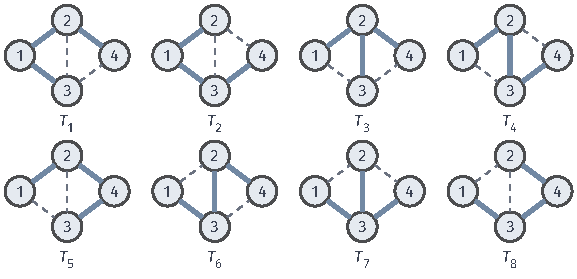
\includegraphics[width=97.652mm]{figures/01-basic-mathematics/04-graphs/tikz/c1-spanning-trees/figure.pdf}
  \caption{贯穿图的全部$8$棵生成树。蓝色粗线是树边，灰色虚线是被舍弃的原边。每棵生成树都有$3$条边并覆盖全部$4$个顶点；从$5$条边中选$3$条的$10$种选法里，只有恰好组成三角形$\{1,2,3\}$或$\{2,3,4\}$的两种不是树。}
  \label{fig:graph-conn-spanning-trees}
\end{figure}

生成树舍弃了环所提供的替代路径。以$T_2$为例：原图中$2,4$相邻，在$T_2$中却要经过$(2,1,3,4)$；原图没有割点，而$T_2$中$1$和$3$都成了割点。所以生成树上的距离和脆弱性一般不等于原图上的结果。生成森林恰好用最少的边给出第~\ref{sec:graph-conn-components}小节核对分量划分所需的块内连接。用遍历求生成森林是第~\ref{sec:graph-connectivity-computation}节的内容，它只保证连通、不比较边权；带建设成本时选总成本最小的一棵，是第~\ref{sec:graph-minimum-spanning-tree}章的问题。

\subsection{二部图}
\label{sec:graph-bipartite-graphs}

人员与岗位配对、用户与商品推荐、或者变量节点与局部函数因子相连（第~\ref{chap:local-functions-tree-dp}章）时，顶点天然分成两类，所有的边都只连接不同类的顶点，同类顶点之间绝不连边。这种二部结构是第~\ref{chap:bipartite-matching-assignment}章匹配与指派问题的舞台。

\begin{definition}[二部图与完全二部图]
\label{def:graph-bipartite}
设$\mathcal G=(V,E)$是无向图。若顶点集$V$可以划分为两个互不相交的子集$X$和$Y$（$V=X\cup Y$，$X\cap Y=\varnothing$），使得$E$中每条边都有一个端点在$X$中、另一个端点在$Y$中，就称$\mathcal G$为\term{二部图}（bipartite graph），称$(X,Y)$为$\mathcal G$的一个二部划分。若进一步地，$X$中每个顶点与$Y$中每个顶点之间都有边相连，就称$\mathcal G$为\term{完全二部图}（complete bipartite graph）；当$|X|=r$、$|Y|=s$时记作$K_{r,s}$，它共有$r+s$个顶点和$rs$条边。
\end{definition}

按第~\ref{sec:graph-cliques-independent-sets}小节的语言，二部划分$(X,Y)$要求$X$和$Y$内部都没有边，即$X$与$Y$都是独立集。如果给$X$中顶点染颜色$1$、$Y$中顶点染颜色$2$，每条边的两个端点颜色都不同，因此二部图就是可以用两种颜色完成正常顶点着色的图（第~\ref{sec:graph-coloring}节将讨论一般图的正常顶点着色与色数$\chi(\mathcal G)$）。任何树都是二部图：任选一个根$r$，按每个顶点到$r$的唯一路径长度的奇偶性将顶点分成两组，树中每条边都连接父节点与子节点，路径长度恰差$1$，两端奇偶性必然相反。

对于没有预先给出分类标签的一般图，怎样判断它能不能做二部划分？如果在图上沿一条路径一步步交替染上蓝、黄两种颜色，走偶数步回到起点时颜色刚好衔接；一旦图中有一个长度为奇数的环，绕环一圈回到起点时，起点的颜色就会与自身发生冲突（图~\ref{fig:graph-bipartite-odd-cycle}）。下面的基本定理证明，有奇环不仅是二部划分失败的常见原因，更是唯一的障碍。

\begin{theorem}[二部图的奇环判别]
\label{thm:graph-bipartite-odd-cycle}
无向图$\mathcal G=(V,E)$是二部图，当且仅当$\mathcal G$中不含长度为奇数的环。
\end{theorem}

\begin{proof}
先证必要性。设$\mathcal G$是二部图，二部划分为$V=X\cup Y$。任取$\mathcal G$中的一个环$C=(v_0,v_1,\ldots,v_{k-1},v_0)$，不妨设$v_0\in X$。因为每条边的两端分别在$X$和$Y$中，沿环依次前进时顶点在$X$与$Y$之间严格交替：当下标$r$为偶数时$v_r\in X$，当$r$为奇数时$v_r\in Y$。特别地，终点$v_k=v_0\in X$，所以环的长度$k$必为偶数，即$\mathcal G$不含奇环。

再证充分性。设$\mathcal G$不含奇环。一张图是二部图当且仅当它的每个连通分量都是二部图，因此不妨设$\mathcal G$连通。任取一个基准顶点$s\in V$，对每个顶点$v\in V$，定义$\delta(v)$为从$s$到$v$的所有行走（等价地，简单路径）中的最小长度，并按$\delta(v)$的奇偶性把$V$划分为
\[
X=\bigl\{v\in V:\delta(v)\text{ 为偶数}\bigr\},\qquad
Y=\bigl\{v\in V:\delta(v)\text{ 为奇数}\bigr\}.
\]
显然$X\cap Y=\varnothing$且$X\cup Y=V$。假设存在一条边$\{u,v\}\in E$，其两端落入同一部分，即$\delta(u)$与$\delta(v)$奇偶性相同。分别取从$s$到$u$的最短路径$P_u$（长度为$\delta(u)$）和从$s$到$v$的最短路径$P_v$（长度为$\delta(v)$）。因为两条路径都以$s$为起点，可以取它们最后一个公共顶点$w$。$P_u$与$P_v$从$s$到$w$的前段都是从$s$到$w$的最短路径，长度都等于$\delta(w)$；而$P_u$从$w$到$u$的后段（长$\delta(u)-\delta(w)$）与$P_v$从$w$到$v$的后段（长$\delta(v)-\delta(w)$）除公共起点$w$外没有其他公共顶点。将这两段路径连同边$\{u,v\}$拼在一起，就得到一个简单环，其长度为
\[
\bigl(\delta(u)-\delta(w)\bigr)+\bigl(\delta(v)-\delta(w)\bigr)+1
=\delta(u)+\delta(v)-2\delta(w)+1.
\]
由于$\delta(u)$与$\delta(v)$奇偶性相同，$\delta(u)+\delta(v)-2\delta(w)$是偶数，加上$1$后该环的长度为奇数，与$\mathcal G$不含奇环矛盾。因此没有任何边的两端落在同一部分中，$(X,Y)$就是$\mathcal G$的二部划分。
\end{proof}

\begin{figure}[!htb]
  \centering
  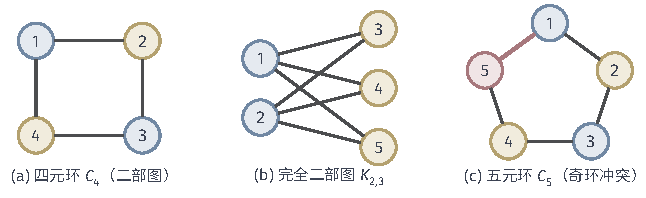
\includegraphics[width=109.432mm]{figures/03-graphs/01-structure-and-computation/tikz/graph-bipartite-odd-cycle/figure.pdf}
  \caption{二部图与奇环障碍。(a)偶环$C_4$按蓝$X=\{1,3\}$、黄$Y=\{2,4\}$交替赋色，每条边两端异色；(b)完全二部图$K_{2,3}$左部与右部之间两两连边，同侧无边；(c)奇环$C_5$从顶点$1$起沿环交替染蓝、黄两色，走到第$5$个顶点时无论染哪一色都会与相邻顶点$4$或$1$同色（红色粗边标出冲突）。}
  \label{fig:graph-bipartite-odd-cycle}
\end{figure}

贯穿图\eqref{eq:graph-conn-running-graph}含有三角形$(1,2,3,1)$，长度为$3$是奇数，由定理~\ref{thm:graph-bipartite-odd-cycle}立即断定它不是二部图；若删去中间边$\{2,3\}$，剩下的四元环$(1,2,4,3,1)$不含奇环，按$X=\{1,4\}$、$Y=\{2,3\}$即可完成二部划分。定理~\ref{thm:graph-bipartite-odd-cycle}充分性的证明完全是构造性的：最短路径边数$\delta(v)$恰是第~\ref{sec:graph-bfs}节广度优先遍历算出的层数，第~\ref{sec:graph-bfs-bipartite}小节将据此给出在$O(n+m)$时间内完成二部图判定或提取奇环的算法。

\subsection{平面图}
\label{sec:graph-planar-graphs}

第~\ref{sec:graph-conn-definition}小节在区分“图的数据”与“图的画法”时指出，贯穿图\eqref{eq:graph-conn-running-graph}既可以画成图~\ref{fig:graph-conn-running-drawings}(c)那样有两条对角边交叉，也可以把其中一条边移到外侧，画成图~\ref{fig:graph-conn-running-drawings}(a)(b)那样没有任何边相交。在印制电路板布线、城市道路网或有限元网格剖分中，边的交叉意味着必须架设跨线桥或增加导电层，于是自然要问：哪些图本身允许在平面上不交叉地画出来？

\begin{definition}[平面图、平面嵌入与面]
\label{def:graph-planar}
设$\mathcal G=(V,E)$是无向图。若能把$V$中各顶点画成平面$\mathbb R^2$上互不相同的点，把$E$中每条边画成连接其两端点的简单曲线，曲线内部不经过任何顶点，并使任意两条边除公共端点外互不相交，就称$\mathcal G$是\term{平面图}（planar graph），这样的一幅具体画法称为$\mathcal G$的一个平面嵌入（或已嵌入的平面图）。

平面嵌入中的点和曲线把平面其余部分分割成若干个极大的连通开区域，每个区域称为该平面嵌入的一个\term{面}（face），其中唯一无界的那个外部区域称为外部无限面（或无穷面）。
\end{definition}

数一个平面嵌入的面数$f$时，有界的内部区域与外部无限面都要计入。例如贯穿图的无交叉画法（图~\ref{fig:graph-planar-euler-k5-k33}(a)）中，两个三角形分别围出有界面$F_1,F_2$，外围四元环$(1,2,4,3,1)$外侧是无界面$F_3$，共有$f=3$个面。不难算得，此时$n-m+f=4-5+3=2$。下面的欧拉公式表明，无论连通平面图长什么样、采取哪种无交叉画法，这个交替和恒等于$2$。

\begin{theorem}[平面图的欧拉公式]
\label{thm:graph-euler-planar}
设连通平面图$\mathcal G=(V,E)$的某个平面嵌入有$n$个顶点、$m$条边和$f$个面，则
\begin{equation}
n - m + f = 2.
\label{eq:graph-euler-planar}
\end{equation}
\end{theorem}

\begin{proof}
固定顶点数$n\geq 1$，对边数$m$作数学归纳法。因为$\mathcal G$连通，由第~\ref{sec:graph-trees-forests}小节可知$m\geq n-1$。

当$m=n-1$时，由定理~\ref{thm:graph-conn-connected-tree-test}，$\mathcal G$是一棵树。树中没有任何环，平面嵌入的曲线不会围出任何有界区域，整个平面只有一个无界的外部面，即$f=1$。此时
\[
n - m + f = n - (n-1) + 1 = 2,
\]
公式成立。

设$m\geq n$，并假设公式对一切有$n$个顶点、$m-1$条边的连通平面图成立。因为$m\geq n$，$\mathcal G$不是树，必含至少一个环$C$。在环$C$上任取一条边$e$。由定理~\ref{thm:graph-conn-bridge-cycle}，$e$不是桥，故删去$e$后$\mathcal G-e$仍然连通，有$n$个顶点和$m'=m-1$条边。在平面嵌入中，环$C$是一条简单闭合曲线，把平面分成内外两侧，边$e$作为$C$上的一段，两侧紧挨着两个不同的面；删去边$e$就打通了这道隔墙，使原来分居$e$两侧的两个面合并成一个面，其余的面保持不变，所以$\mathcal G-e$的面数为$f'=f-1$。对$\mathcal G-e$应用归纳假设，得
\[
n - (m-1) + (f-1) = 2,
\]
整理即得$n - m + f = 2$。由数学归纳法，式\eqref{eq:graph-euler-planar}对一切连通平面图成立。
\end{proof}

欧拉公式告诉我们，连通平面图的面数$f=m-n+2$完全由顶点数和边数决定，与平面嵌入的具体画法无关。更进一步，对含环的连通简单平面图，每个面的边界长度至少为三（不含三角形时至少为四），欧拉公式直接限制了简单平面图最多能有多少条边。

\begin{theorem}[平面图的边数上界]
\label{thm:graph-planar-edge-bound}
设$\mathcal G=(V,E)$是有$n\geq 3$个顶点、$m$条边的简单平面图，则
\begin{equation}
m \leq 3n - 6;
\label{eq:graph-planar-edge-bound}
\end{equation}
若$\mathcal G$中不含三角形（长度为$3$的环），则进一步有
\begin{equation}
m \leq 2n - 4.
\label{eq:graph-planar-bipartite-bound}
\end{equation}
\end{theorem}

\begin{proof}
若$\mathcal G$不连通，先将各分量分别画在互不相交的区域，再逐次用外部面中的边连接这些分量。新边都是桥，不产生交叉或新的环，且只使$m$增大，因此只需对连通图证明；若$\mathcal G$是树，则$n\geq 3$时$m=n-1\leq 2n-4\leq 3n-6$显然成立。以下设$\mathcal G$连通且至少含一个环。

在$\mathcal G$的一个平面嵌入中，沿着每个面$F$的边界走一圈，所经过的边数称为面$F$的边界长度（桥如果在某个面的内部伸出，沿边界绕过它时会来回经过两次，按两次计）。因为$\mathcal G$是简单图且含有环，每个面的边界都至少包含一个环，而在简单图中环长至少为$3$，所以每个面的边界长度都至少为$3$。把全部$f$个面的边界长度加起来：每条非桥边恰好分隔两个面，在两个面的边界上各算一次；每条桥在包含它的那个面的边界上往返算两次。因此所有面的边界长度之和恰好等于$2m$，从而
\[
2m \geq 3f.
\]
由欧拉公式\eqref{eq:graph-euler-planar}代入$f = 2 - n + m$，得
\[
2m \geq 3(2 - n + m) = 6 - 3n + 3m,
\]
移项即得$m \leq 3n - 6$。

当$\mathcal G$不含三角形时，任何环的长度至少为$4$，从而每个面的边界长度都至少为$4$。同样的计数给出$2m \geq 4f = 4(2 - n + m)$，整理即得$2m \leq 4n - 8$，即$m \leq 2n - 4$。
\end{proof}

\begin{figure}[!htb]
  \centering
  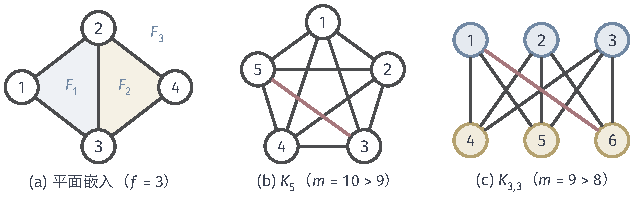
\includegraphics[width=107.361mm]{figures/03-graphs/01-structure-and-computation/tikz/graph-planar-euler-k5-k33/figure.pdf}
  \caption{平面图的面计数与两张基本非平面图。(a)贯穿图的平面嵌入有$n=4$个顶点、$m=5$条边，围出两个有界面$F_1,F_2$与外部无限面$F_3$，满足$4-5+3=2$；(b)完全图$K_5$有$10$条边，超过平面图上限$3n-6=9$；(c)完全二部图$K_{3,3}$不含奇环从而无三角形，其$9$条边超过无三角形平面图上限$2n-4=8$，二者都无法消除边交叉。}
  \label{fig:graph-planar-euler-k5-k33}
\end{figure}

定理~\ref{thm:graph-planar-edge-bound}立即可用来证明完全图$K_5$和完全二部图$K_{3,3}$（图~\ref{fig:graph-planar-euler-k5-k33}(b)(c)）都不是平面图。对$K_5$，顶点数$n=5$，边数$m=\binom52=10$；若它是平面图，由式\eqref{eq:graph-planar-edge-bound}应有$m\leq 3\times 5-6=9$，与$m=10$矛盾，所以$K_5$不是平面图。对$K_{3,3}$，顶点数$n=6$，边数$m=3\times 3=9$，只代式\eqref{eq:graph-planar-edge-bound}给出$9\leq 3\times 6-6=12$，还看不出矛盾；但$K_{3,3}$是二部图，由定理~\ref{thm:graph-bipartite-odd-cycle}它不含任何奇环，特别地不含三角形，故必须满足更紧的式\eqref{eq:graph-planar-bipartite-bound}，即$m\leq 2\times 6-4=8$，与$m=9$矛盾，所以$K_{3,3}$也不是平面图。Kuratowski定理进一步证明，$K_5$与$K_{3,3}$正是平面性的全部障碍：一张有限图是平面图，当且仅当它不包含任何由$K_5$或$K_{3,3}$在边上插入度为$2$的细分顶点所得的子图。

\paragraph{平面图的对偶与地图着色}
给定连通平面图$\mathcal G$的一个平面嵌入，可以在每个面$F_i$内部各放一个对偶顶点$f_i^*$，对原图的每条边$e$，连接其两侧面的对偶顶点，并使这条对偶边$e^*$穿过$e$。若$e$是桥，两侧为同一面，对偶边就是自环；不同原边也可能产生平行对偶边。因此，对偶图$\mathcal G^*$一般是允许自环和平行边的平面多重图。在地图着色问题中，要求共享边界线的相邻行政区染不同颜色，等价于对平面嵌入的面做正常着色，相应地，要对删去自环并合并平行边后的对偶简单图作正常顶点着色；自环不表示两个不同区域之间的邻接。一般顶点着色见第~\ref{sec:graph-coloring}节。

对$n\geq3$的简单平面图，由式\eqref{eq:graph-planar-edge-bound}结合度数和公式\eqref{eq:graph-conn-handshake}，度数和满足
\[
\sum_{i\in V}d_i = 2m \leq 6n - 12 < 6n,
\]
这意味着平均度严格小于$6$，图中存在度不超过$5$的顶点。$n=1,2$时此结论可直接核对，因此它对所有非空简单平面图成立。删去$v$对剩余平面图递归着色后再把$v$放回，当$d_v\leq 4$时直接有空余颜色，当$d_v=5$时借助双色交替路径交换颜色即可证明任何平面图都可用不超过$5$种颜色使相邻顶点异色（五色定理）；而更精细的归约与构形分析给出了著名的四色定理，即一切简单平面图都可用不超过$4$种颜色完成正常顶点着色（第~\ref{sec:graph-coloring}节）。
